\documentclass[14pt,final]{report}
\usepackage[english,russian]{babel}

% TODO: Do something 
% https://www.overleaf.com/read/fkzbbcxxrxvz
% This was edited locally
% And this was edited on the server

% \RequirePackage{polyglossia}
% \setotherlanguage{english}
% \setdefaultlanguage{russian}

\RequirePackage[times,firacode,a4paper,microtyping,732,smalltitles,listbib,lmmath]{subook}
% \RequirePackage[times,firacode,a4paper,microtyping,handbook,smalltitles,listbib]{subook}
\RequirePackage{tabularx}
% \RequirePackage{grphicx}
\graphicspath{{/pics}}

\usepackage[T1]{fontenc}

\catcode`_=12
\begingroup\lccode`~=`_\lowercase{\endgroup\let~\sb}
\mathcode`_="8000

% \usepackage{showframe}

% pygmetize
\RequirePackage{minted}
\usemintedstyle{tango} % bw

% \setmainfont{Times New Roman}

\begin{document}
\thispagestyle{empty}
\begin{center}
МИНИСТЕРСТВО ОБРАЗОВАНИЯ И НАУКИ РОССИЙСКОЙ ФЕДЕРАЦИИ

Федеральное государственное бюджетное образовательное учреждение высшего образования

«ИРКУТСКИЙ  ГОСУДАРСТВЕННЫЙ УНИВЕРСИТЕТ»\\
(ФГБОУ ВО «ИГУ»)
\end{center}
\vfill % \vfil \vfill \vfilll

\noindent\begin{tabularx}{\textwidth} {
  >{\raggedright\arraybackslash}X
  >{\raggedright\arraybackslash}X }
Институт математики и информационных технологий
&
Кафедра информационных технологий
\end{tabularx}

\vfill
\begin{center}
  \textbf{ОТЧЕТ}
\vspace{1em}

о курсовой работе по курсу <<Разработка WEB-приложений>>

{\bf Разработка REST API для мессенджера}

\end{center}
\vfill

\noindent\begin{tabularx}{\textwidth} {
  >{\raggedright\arraybackslash}X
  >{\raggedright}X }
&

Студента 3 курса группы 2371--ДБ\\
Чехова Александра Игоревича\\
Направление\;: 02.03.02--~Фундаментальная информатика и информационные технологии\\[2em]

Руководитель:\\
канд.~техн.~наук доцент\\
Черкашин Евгений Александрович\\[2em]

Курсовая работа защищена с оценкой\\[1em] \underline{\hspace{3cm}}
\end{tabularx}
\vfill
\begin{center}
  Иркутск -- 2021
\end{center}
\clearpage

\tableofcontents

\chapter*{ВВЕДЕНИЕ}
% TODO: Add contents line
\label{chap:intro}

Целью данной курсовой работы была поставлена разработка веб--приложения --- приложение, клиентом которой будет страница в браузере (клиент). Конкретной темой и целью для приложения был выбран мессенджер (М). Суть М состоит в предоставлении возможности обмена текстовыми сообщениями между пользователями.

Такому приложению необходимо постоянно взаимодействовать с сервером: получать и отправлять данные. Для создаваемого М разработан REST API, позволяющий взаимодействовать с базой данных (БД) путём получения запросов от клиента. В данном отчёте представлены результаты разработки именно этой части приложения.

Учитывая учебную направленность данной работы, были сформулированы следующие требования к серверному приложению:
\begin{itemize}
    \item Смоделировать интерфейс допустимых запросов (API);
    \item Спроектировать и создать БД;
    \item Смоделировать и задать необходимые запросы к БД;
    \item Разработать обработку запросов от клиентов (маршрутизацию);
\end{itemize}

Так же, исходя из поставленных задач необходимо выбрать БД и фреймворк для реализации маршрутизации. Фреймворк должен обеспечить удобное и лёгкое создание серверного приложения, так как целевое приложение не имеет особых требований к API. БД в свою очередь должна предоставить удобный формат хранения данных. Так как это курсовая работа в рамках обучения, в качестве указанных выше программных инструментов были выбраны те, что рассчитаны на малую нагрузку --- число обрабатываемых запросов.

\chapter{Теоретические основы разработки REST API}

Большинство приложений использующих интернет сети полагаются на сервера --- компьютеры, позволяющие использовать свои ресурсы (аппаратные мощности) и данные другим компьютерам в локальной или глобальной сети. Такую архитектуру часто определяют как клиент--серверной: клиент совершает запросы к серверу и получает ответы в виде данных и/или подтверждений записи данных из запроса \cite{snaider}.

Для обработки запросов на сервере могут создаваться как большие изолированные программы, так и маленькие, предназначенные для простых целей, при чём вторые могут запускаться как отдельно, так и в составе первых.

Для обработки запросов такого приложения как мессенджер будет достаточно и небольшого приложения. Данное приложение должно позволять: 
\begin{itemize}
    \item считывать получаемые компьютером по сети Итернет запросы и приходящие с ними данные,
    \item легко подключаться к базе данных (БД),
    \item отправлять ответные данные клиенту и статус коды --- зарезервированные числовые комбинации, несущие информацию о состоянии обработки запроса,
\end{itemize}

В качестве запросов выступают посланные данные на сервер данные по определённому протоколу --- HTTP\cite{polard}. Сервер считывает эти данные и направляет данные к приложению, которому они назначаются, а тот в свою очередь схожим образом отправляет ответ клиенту. Во многих случаях запросы схожи с ссылками на сайты, которые пользователи вводят в адресной строке браузера. Такое поведение обеспечивают DNS--сервера, которые производят связывание текстовых ссылок с определёнными компьютерами, и серверами в частности. Именно эту возможность и будет использовать разрабатываемое REST API приложение --- по своей сути оно является отражением этой идеи на практике: приложение позволяет делать к себе HTTP-запросы и выдаёт ответы.

Сама программа представляет из себя множество методов, которые обрабатывают определённые команды, приходящие в запросе клиента. Такие программы предоставляют определённый интерфейс воздействия на них и их состояние, из-за чего клиент должен знать как именно нужно делать запросы, чтобы программа выполнила их на сервере и ответила необходимыми данными.

Так же серверные приложения часто используют базы данных для хранения информации пользователя, о пользователе или просто для выдачи её при необходимых условиях (оплате, членстве клуба и т.\,п.). Одним из видов БД являются SQL подобные БД. Такие БД хранят ифнформацию в виде таблиц и поддерживают различные отложения между записями в таблицах.

Между приложением и БД так же необходима программная связь которая обеспечит удобный интерфейс добавления данных в БД и их чтения от туда же. Это необходимо потому, что большинство разработчиков БД стремятся к улучшению функциональности БД, а следственно и добавлению особенностей. Программа--коннектор обеспечит обработку всех особенностей выбранной БД.

После изучения предметной области --- приложение--мессенджер, выделены основные операции производимые пользователями:
\begin{itemize}
    \item Отправка сообщения,
    \item Получение сообщений из диалога с одним из других пользователей,
    \item Добавление новых пользователей в список контактов,
    \item Авторизация.
\end{itemize}
Также отдельно стоит упомянуть операцию регистрацию --- нерегулярное действие, но требующее всей ответственности работы с запросом и БД.

Реализацию операций описанных выше можно считать требованиями к проекту --- всему веб--приложению в целом.


\chapter{Реализация REST API Приложения}

\section{Моделирование API}

После изучения требований к веб--приложению было необходимо задать виды ссылок, по которым клиентская часть приложения будет делать запросы на серверную. В результате заданы следующие ссылки:
\begin{itemize}
    \item \texttt{/get_massages} --- получение сообщений диалога,
    \item \texttt{/getuser} --- получение информации о пользователи для создания нового диалога,
    \item \texttt{/send_massage} --- отправка сообщения,
    \item \texttt{/login} --- для авторизации,
    \item \texttt{/register} --- регистрация,
    \item \texttt{/renew_name} --- изменение имени,
    \item \texttt{/renew_avatar} --- изменение аватара (картинки в профиле).
\end{itemize}
Последние два пункта позволяют клиенту реализовать функционал, повышающий удобство использования приложения: человеку проще идентифицировать себя и других людей картинкой и именем, которые они могут менять под себя.

\section{Проектирование БД}
В системе мессенджера имеются две сущности: пользователи и сообщения. Так же необходимо хранить связи пользователей друг с другом, как участников диалогов. В связи с этими условиями была выбрана сдледующая архитектура БД:
\begin{figure}[hbtp]
  \centering
  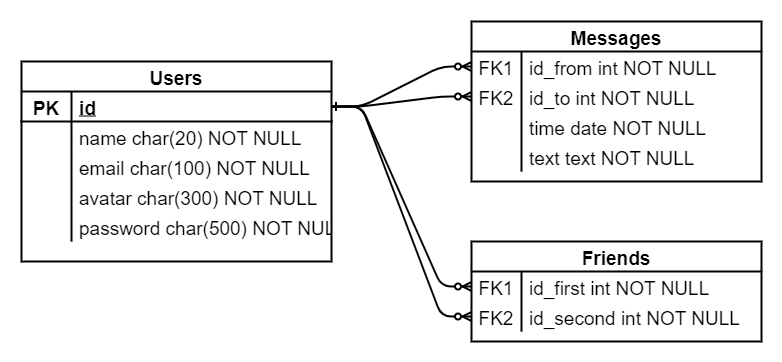
\includegraphics[width=0.7\linewidth]{pics/db.png}
  \caption{Диаграмма отношений таблиц базы данных}
  \label{fig:db}
\end{figure}

В качестве базы данных была выбрана SQLite. Эта БД представляет из себя просто файл, который можно использовать как SQL-подобную БД. Из-за этого SQLite является простой в настройке, малой по объёму занимаемой памяти, но в качестве минуса скорость работы --- что не выходит за рамки требований к учебному проекту.

\section{Язык программирования и его библиотеки}
В качестве языка программирования для разработки приложения был выбран Python \cite{barry}. Под этот язык разработано много удобных и мощных библиотек, помогающих решать большие задача, без необходимости писать большие объёмы кода.

\section{Основной фреймворк для создания приложения}
В качестве основы выбран легковесный фреймворк \texttt{Flask} \cite{grinberg}.

\texttt{Flask} --- это фреймворк, позволяющий создать простое серверное приложение с базовым функционалом:
\begin{itemize}
    \item Обработка \texttt{HTTP} запросов,
    \item Подключение к БД,
    \item Возврат по значений из БД.
\end{itemize}
При создании простого REST API для мессенджера этого будет вполне достаточно.

Во \texttt{Flask}, первым делом, создаётся объект приложения (см. приложение листинг \ref{lst:app}). Также сразу удобно задать в конфиге приложения переменную \texttt{SQLALCHEMY_DATABASE_URI}. Такая настройка позволит удобно использовать другую библиотеку (её модифицированную под \texttt{Flask} версию). 

На данном этапе имеется представление сруктуры БД. Рассмотрим создание её структуры и запросов к ней для более удобного дальнейшего понимания релизации обработчиков запросов.

\section{Алгоритм порождения структуры базы данных}
\label{sec:struct-bd}

Главной библиотекой, помогающей работать с БД стара \texttt{sqlalchemy}, а точнее \texttt{flask_sqlalchemy}. Версия для \texttt{Flask} позволяет автоматизировать некоторые постоянные вещи, как ручное подключение к базе данных, создание состояния для каждого запроса и проведение этого состояния через все запросы к самой БД. Но такое упрощение не обходится без ограничений, по этому и обычная \texttt{sqlalchemy} понадобится, например при создании сложных запросов (см. приложение листинг \ref{lst:db1}).

После того, как была задана конфигурационная переменная для приложения, остаётся три шага:
\begin{enumerate}
    \item Создать объект класса \texttt{SQLalchemy} --- переменная \texttt{db}, передав ей объект приложения,
    \item Воссоздать структуру БД в виде соответствия каждой таблице класса, наследующегося от \texttt{db.Module}
    \item Вызвать метод \texttt{db.create_all()} (см. приложение листинг \ref{lst:start}), который, ориентируясь на проделанные ранее шаги, создаст базу данных и необходимые таблицы в ней.
\end{enumerate}
В результате выполнения этих шагов в дирректории проекта появился файл \texttt{messanger.db}, который и представляет БД. 

\section{Создание запросов к БД}
После проектирования БД, нужно установить те операции с данными внутри неё, которые будут проделываться в будущем. Анализируя требования к проекту можно выделить следующие операции:
\begin{itemize}
    \item Добавление пользователя,
    \item Добавление сообщения,
    \item Добавление связи связи двумя пользователям
    \item Получение информации о пользователе по его \texttt{id} / \texttt{email}
    \item Получение сообщений между двумя пользователями
    \item Получение друзей пользователя --- других пользователей, с которыми он связан
\end{itemize}
Все эти операции разработаны в виде функций, которые уже реализуют запросы к БД (см. приложение листинги \ref{lst:db2}--\ref{lst:db5}). Все функции реализуют схожий алгоритм: 
\begin{enumerate}
    \item В блоке \texttt{try} проделываются необходимые операции: проверки и изъятия информации,
    \item В блоке \texttt{except} отлавливаются возможые ощибки при работе с БД,
    \item В блоке \texttt{finaly} закрывается ссеся подключения к БД.
\end{enumerate}
Все представленные функции позволяют при маршрутизации не задумываться о том, как и от куда берутся данные.

\section{Реализация маршрутизации}
Все функции маршрутизации --- это функции, обёрнутые в декораторы вида \texttt{@app.route()} (см. приложение листинги \ref{lst:route1}--\ref{lst:route3}). Аргументом такому декораторам передаётся строка, которую будет необходимо прописать клиенту при запросе. Так же можно передать массив методов запросов, которые будет принимать приложение. В итоге получился набор функций которые обрабатывают определённые запросы и выполняет соответствующие действия. Все функции с запросом получают JSON--объекты, из которых извлекают необходимую информацию. При неудаче: некорректные данные, отказе в доступе или информации нет -- функции возвращают код 400, иначе код 200.

\begin{table}[h]
    \centering
    \begin{tabular}{|p{3cm}|p{3cm}|p{10cm}|}
        \hline
        Функция & Запрос & Выполняемое действие \\ \hline
        \texttt{register()} & \texttt{/register} & Исходя из полученной информации добавляет нового пользователя в БД \\ \hline
        \texttt{login()} & \texttt{/login} & Проверяет верность полученных данных: email и пароль, и возвращает коды 200 если всё верно  \\ \hline
        \texttt{get_messages()} & \texttt{/get_messages} & Возвращает все сообщения между двумя пользователями, идентефикаторы которых получены в зпросе \\ \hline
        \texttt{get_user()} & \texttt{/get_user} & Возвращает информацию о пользователе, email которого был получен в запросе \\ \hline
        \texttt{add_message()} & \texttt{/send_message} & Добовляет собщение в БД \\ \hline
        \texttt{renew_name()} & \texttt{/renew_name} & Обновляет имя пользователя на полученное \\ \hline
        \texttt{renew_avatar()} & \texttt{/renew_avatar} & Обновляет аватарку пользователя (сохраняет новыую ссылку на картинку из интернета) \\ \hline
    \end{tabular}
    \caption{Функции маршрутизации}
    \label{tab1}
\end{table}

Так же имеется метод \texttt{shut_down_connection()}, который после обработки каждого запроса закрывает сессию подключения к БЗ (дополнительная мера предосторожности).

\chapter*{ЗАКЛЮЧЕНИЕ}
По итогу проделанной работы было разработано веб-приложение представляющее из себя простой мессенджер, и позволяющее пользователям:
\begin{itemize}
    \item Регистрироваться и авторизоваться в системе,
    \item Отправлять друг другу сообщения,
    \item Добавление новых пользователей в список контактов,
    \item Изменять имя и аватарку в профиле.
\end{itemize}
В частности серверная часть приложения предоставляется API для обработки соответсвующих запросов с клиента.

Созданное веб-приложение можно доработать следующими пунктами:
\begin{itemize}
    \item Получение сообщения без необходимости перезагрузки всего диалога
    \item Возможность отправки файлов (картинок, аудио и др.)
    \item Возможность удаления сообщений и контактов
    \item Отправку уведомлений в браузере
    \item Зашифрованная передача сообщений
    \item Наличие отдельных таблиц в базе данных (БД) для хранения персональных данных
\end{itemize}

По результатам работы над курсовым проектом был получен опят разработки REST API приложения при помощи языка программирования \texttt{Python} и библиотеки \texttt{Flask}. Также была спроектирована БД и изучена работа с библиотекой \texttt{SQLalchemy}, позволяющей воссоздавать структуру БД из создаваемых \texttt{Python}--классов и делать различные запросы к БД.

\begin{thebibliography}{99}
\bibitem{snaider} Cнейдер Й. Эффективное программирование TCP/IP: Пер. с англ. -- М.: ДМК Пресс.-- 320 с.
\bibitem{polard} Поллард Б. HTTP/2 в действии / пер. с анг. П. М. Бомбаковой.-- М.: ДМК Пресс, 2021.-- 424 с.
\bibitem{barry} Бэрри, Пол Изучаем программирование на Python / пер. с англ. М. А. Райтман.-- М.: Эскимо, 2020.-- 624 с.
\bibitem{grinberg} Гринберг М. Разработка веб-приложений с использованием Flask на языке Python / пер. с анг. А. Н. Киселева.-- М.: ДМК Пресс, 2014.-- 272 с.
\end{thebibliography}

\appendices

\chapter{Исходный код программ}

\begin{listing}[htbp]
\begin{center}
{\footnotesize
\begin{verbatim}
DB_CONFIG = {               # it was for PostgreSQL 
    'user': 'postgres',
    'password': 'su_12345',
    'host': '127.0.0.1',
    'port': '5432',
    'database': 'messeger'}
SQLITE_FILE_NAME = 'messanger.db'
DEBUG = True
DEFAULT_AVATAR = 'https://vraki.net/sites/default/files/inline/images/30_55.jpg'
\end{verbatim}}
\end{center}
\caption{Файл \texttt{config.py}}\label{lst:config}
\end{listing}

\begin{listing}[htbp]
\begin{center}
{\footnotesize
\begin{verbatim}
from config import SQLITE_FILE_NAME
from flask import Flask
app = Flask(__name__)
#app.config['SQLALCHEMY_DATABASE_URI'] = \
#    "postgresql+psycopg2://{user}:{password}@{host}:{port}/{database}".format(**DB_CONFIG)
app.config['SQLALCHEMY_DATABASE_URI'] = f"sqlite:///{SQLITE_FILE_NAME}"
app.config['SQLALCHEMY_TRACK_MODIFICATIONS'] = False
\end{verbatim}}
\end{center}
\caption{Файл \texttt{application.py}}\label{lst:app}
\end{listing}

\begin{listing}[htbp]
\begin{center}
{\footnotesize
\begin{verbatim}
import db_operations
from database import db
from application import app
from config import DEBUG
from flask_cors import CORS
import routing
db_operations.create_db()
db.create_all()
if DEBUG:
    client = app.test_client()
CORS(app)
if __name__ == '__main__':
    app.run(debug=DEBUG)
\end{verbatim}}
\end{center}
\caption{Файл \texttt{start.py}}\label{lst:start}
\end{listing}

\begin{listing}[htbp]
\begin{center}
{\footnotesize
\begin{verbatim}
from application import app
from flask_sqlalchemy import SQLAlchemy
from sqlalchemy import and_, or_
from sqlalchemy.sql import func
from datetime import datetime
from werkzeug.security import generate_password_hash, check_password_hash
from config import DEFAULT_AVATAR

db = SQLAlchemy(app)


class Users(db.Model):
    id = db.Column(db.Integer, primary_key=True)
    name = db.Column(db.String(20), nullable=False)
    email = db.Column(db.String(100), nullable=False, unique=True)
    avatar = db.Column(db.String(300), nullable=True)
    password = db.Column(db.String(500), nullable=False)

    def as_dict(self):
        return {'id': self.id,
                'avatar': self.avatar if self.avatar else DEFAULT_AVATAR,
                'name': self.name}

    def __repr__(self):
        return f"<users {self.id}>"


class Friends(db.Model):
    first_id = db.Column(db.Integer, db.ForeignKey('users.id'),
                         primary_key=True)
    second_id = db.Column(db.Integer, db.ForeignKey('users.id'),
                          primary_key=True)

    def __repr__(self):
        return f"<friends {self.first_id} : {self.second_id}>"


class Messages(db.Model):
    id_from = db.Column(db.Integer, db.ForeignKey('users.id'),
                        primary_key=True)
    id_to = db.Column(db.Integer, db.ForeignKey('users.id'),
                      primary_key=True)
    time = db.Column(db.DateTime(timezone=False), primary_key=True,
                     default=func.now())
    text = db.Column(db.Text, nullable=False)

    def as_dict(self):
        return {'id_from': self.id_from,
                'id_to': self.id_to,
                'time': self.time.timestamp(),
                'text': self.text}

    def __repr__(self):
        return f"<Messages {self.id_from} -> {self.id_to}>"

\end{verbatim}}
\end{center}
\caption{Файл \texttt{database.py}, часть 1}\label{lst:db1}
\end{listing}

\begin{listing}[htbp]
\begin{center}
{\footnotesize
\begin{verbatim}
def add_user(name, email, password):
    try:
        if (Users.query.filter(Users.email == email)).all():
            return False
        u = Users(name=name, email=email,
                  password=generate_password_hash(password))
        db.session.add(u)
        db.session.flush()
        db.session.commit()
        return True
    except Exception as e:
        db.session.rollback()
        print(e)
        print('Не удалось добавить пользователя')
        return False
    finally:
        db.session.remove()


def add_message(id_from, id_to, text):
    try:
        if len(Users.query.filter(or_(Users.id == id_from,
                                      Users.id == id_to)).all()) != 2:
            return False

        m = Messages(id_from=id_from, id_to=id_to,
                     text=text)
        db.session.add(m)
        db.session.flush()
        db.session.commit()
        return True
    except Exception as e:
        db.session.rollback()
        print(e)
        print('Не удалось добавить сообщение')
        return False
    finally:
        db.session.remove()
\end{verbatim}}
\end{center}
\caption{Файл \texttt{database.py}, часть 2}\label{lst:db2}
\end{listing}


\begin{listing}[htbp]
\begin{center}
{\footnotesize
\begin{verbatim}
def add_friends(first_id, second_id):
    try:
        if len(Users.query.filter(or_(Users.id == first_id,
                                      Users.id == second_id)).all()) != 2 or \
                len(
                    Friends.query.filter(or_(
                        and_(Friends.first_id == first_id, Friends.first_id == second_id),
                        and_(Friends.first_id == second_id, Friends.first_id == first_id))
                    ).all()
                ) != 0:
            return False

        f = Friends(first_id=first_id, second_id=second_id)
        db.session.add(f)
        db.session.flush()
        db.session.commit()
    except Exception as e:
        db.session.rollback()
        print(e)
        print('Не удалось добавить сообщение')
        return False
    finally:
        db.session.remove()


def renew_name(user_id, new_name):
    try:
        user = Users.query.get(user_id)
        if not user:
            return False
        user.name = new_name
        db.session.commit()
        return True
    except Exception as e:
        print(e)
        print('Не удалось обновить имя')
        return False
    finally:
        db.session.remove()
\end{verbatim}}
\end{center}
\caption{Файл \texttt{database.py}, часть 3}\label{lst:db3}
\end{listing}

\begin{listing}[htbp]
\begin{center}
{\footnotesize
\begin{verbatim}
def renew_avatar(user_id, new_avatar):
    try:
        user = Users.query.get(user_id)
        if not user:
            return False
        user.avatar = new_avatar
        db.session.commit()
        return True
    except Exception as e:
        print(e)
        print('Не удалось обновить фото')
        return False
    finally:
        db.session.remove()


def get_user(user_in_list):
    try:
        if not user_in_list:
            return False
        return user_in_list[0]
    except Exception as e:
        print(e)
        print('Не удалось получить пользователя')
    finally:
        db.session.remove()

def get_user_by_email(email):
    return get_user(Users.query.filter(Users.email == email).all())


def get_user_by_id(user_id):
    return  get_user(Users.query.filter(Users.id == user_id).all())


def get_messages(id_1, id_2):
    try:
        if len(Users.query.filter(or_(Users.id == id_1,
                                      Users.id == id_2)).all()) != 2:
            return []
        return Messages.query.filter(or_(
            and_(Messages.id_from == id_1, Messages.id_to == id_2),
            and_(Messages.id_from == id_2, Messages.id_to == id_1))
        ).order_by(Messages.time).all()
    except Exception as e:
        print(e)
        print('Не удалось получить сообщения')
        return []
    finally:
        db.session.remove()
\end{verbatim}}
\end{center}
\caption{Файл \texttt{database.py}, часть 4}\label{lst:db4}
\end{listing}

\begin{listing}[htbp]
\begin{center}
{\footnotesize
\begin{verbatim}
def get_friends(user_id):
    try:
        if not Users.query.filter(Users.id == user_id).all():
            return []
        return Friends.query.filter(or_(Friends.first_id == user_id,
                                    Friends.second_id == user_id)).all()
    except Exception as e:
        print(e)
        print('Не удалось получить друзей')
        return []
    finally:
        db.session.remove()


def check_user(email, password):
    try:
        if len(Users.query.filter(Users.email == email).all()) < 1:
            return False
        return check_password_hash(
            Users.query.filter(Users.email == email).one().password,
            password)
    except Exception as e:
        print(e)
        print('Не удалось получить друзей')
        return []
    finally:
        db.session.remove()
\end{verbatim}}
\end{center}
\caption{Файл \texttt{database.py}, часть 5}\label{lst:db5}
\end{listing}



\begin{listing}[htbp]
\begin{center}
{\footnotesize
\begin{verbatim}
from application import app
import database as db
from flask import request, make_response


@app.route('/get_messages', methods=['POST'])
def get_messages():
    try:
        id_first = request.get_json().get('myId')
        id_second = request.get_json().get('userId')
        messages = [m.as_dict() for m in db.get_messages(id_first, id_second)]
        status_code = 200
    except KeyError:
        messages = []
        status_code = 400
    response = make_response({'messages': messages}, status_code)
    response.headers.add('Access-Control-Allow-Origin', '*')
    return response


@app.route('/get_user', methods=['POST'])
def get_user():
    try:
        email = request.get_json().get('email')
        user_id = request.get_json().get('id')
        friend = db.get_user_by_email(email)
        if friend:
            friend = friend.as_dict()
            db.add_friends(user_id, friend['id'])
            status_code = 200
        else:
            friend = {}
            status_code = 400
    except KeyError:
        friend = {}
        status_code = 400
    response = make_response(friend, status_code)
    response.headers.add('Access-Control-Allow-Origin', '*')
    return response
\end{verbatim}}
\end{center}
\caption{Файл \texttt{routing.py}, часть 1}\label{lst:route1}
\end{listing}


\begin{listing}[htbp]
\begin{center}
{\footnotesize
\begin{verbatim}
@app.route('/send_message', methods=['POST'])
def add_message():
    try:
        id_form = request.get_json().get('id_from')
        id_to = request.get_json().get('id_to')
        text = request.get_json().get('text')
        status_code = 200 if db.add_message(id_form, id_to, text) else 400
    except KeyError:
        status_code = 400
    response = make_response({}, status_code)
    response.headers.add('Access-Control-Allow-Origin', '*')
    return response


@app.route('/login', methods=['POST'])
def login():
    ret = {}
    try:
        req_json = request.get_json()
        email = req_json.get('email')
        password = req_json.get('password')
        status_code = 200 if db.check_user(email, password) else 400
        if status_code == 200:
            user = db.get_user_by_email(email).as_dict()
            user_id = user['id']
            pairs = db.get_friends(user_id)
            if pairs:
                ids1, ids2 = zip(*[[p.first_id, p.second_id] for p in pairs])
                ids = set(ids1 + ids2)
                friends = [db.get_user_by_id(fid).as_dict()
                           for fid in ids if fid != user_id]
            else:
                friends = []
            ret = {'user': user,
                   'friends': friends}
    except KeyError:
        status_code = 400
    response = make_response(ret, status_code)
    response.headers.add('Access-Control-Allow-Origin', '*')
    return response
\end{verbatim}}
\end{center}
\caption{Файл \texttt{routing.py}, часть 2}\label{lst:route2}
\end{listing}

\begin{listing}[htbp]
\begin{center}
{\footnotesize
\begin{verbatim}
@app.route('/register', methods=['POST'])
def register():
    try:
        req_json = request.get_json()
        name = req_json.get('name')
        email = req_json.get('email')
        password = req_json.get('password')
        status_code = 200 if db.add_user(name, email, password) else 400
    except KeyError:
        status_code = 400
    response = make_response({}, status_code)
    response.headers.add('Access-Control-Allow-Origin', '*')
    return response


@app.route('/renew_name', methods=['POST'])
def renew_name():
    try:
        req_json = request.get_json()
        user_id = req_json.get('id')
        new_name = req_json.get('name')
        status_code = 200 if db.renew_name(user_id, new_name) else 400
    except KeyError:
        status_code = 400
    response = make_response({}, status_code)
    response.headers.add('Access-Control-Allow-Origin', '*')
    return response


@app.route('/renew_avatar', methods=['POST'])
def renew_avatar():
    try:
        req_json = request.get_json()
        user_id = req_json.get('id')
        new_avatar = req_json.get('avatar')
        status_code = 200 if db.renew_avatar(user_id, new_avatar) else 400
    except KeyError:
        status_code = 400
    response = make_response({}, status_code)
    response.headers.add('Access-Control-Allow-Origin', '*')
    return response


@app.teardown_appcontext
def shut_down_connection(exception=None):
    if exception:
        print(exception)
    db.db.session.remove()
\end{verbatim}}
\end{center}
\caption{Файл \texttt{routing.py}, часть 3}\label{lst:route3}
\end{listing}










\end{document}




%%% Local Variables:
%%% mode: latex
%%% TeX-master: t
%%% End:
